\section{Introduction}
\label{sec:introduction}
Reducing inference cost requires models whose computations can be executed
efficiently. Activation sparsity is one approach: when an input is zero, its
contribution to a multiplication is known, creating an opportunity to avoid
work. The useful opportunity depends on both the number of zeros and the
operations they enter. A sparse feed-forward hidden state affects one
projection; sparse inputs to attention and feed-forward projections affect
other matrix products; sparse queries, keys, and values can also affect the
attention products. Training determines how much of this sparsity a model can
accommodate at a given prediction quality.

Existing work approaches this problem from several directions. Training-free
methods remove small activations from a fixed model
\citep{liu2024teal,lee2024cats}. Training interventions introduce or encourage
sparsity, often through feed-forward activations
\citep{mirzadeh2023relu,song2024prosparse,zhang2024exploring}.
Broader approaches already include all linear inputs, structured masks, and
end-to-end execution \citep{wang2024qsparse,you2025spark,cetin2026sparser}.
These advances make a more specific scientific question useful:
\emph{how does the effect of sparsity pressure change when the set of gated
activations changes?} Answering it requires matched architecture and
optimization comparisons, together with a common accounting of the operations
each intervention can affect.

We investigate this question with an intervention ladder containing controlled
branches. At 14M parameters, we first vary pressure on the feed-forward hidden
state. We then hold a four-site gate configuration fixed while expanding the
pressure sites. Finally, we add sign-preserving gates to attention queries,
keys, and values and compare training with and without pressure within each
gate configuration. These comparisons share initialization, data order, and
training schedule. Each threshold gives a matched contrast; the five
thresholds characterize a dose response under one seed.

The central exploratory finding is that broader pressure has a different effect depending
on where gates are placed. With four gated sites, spreading pressure beyond
the feed-forward hidden state raises loss throughout the tested grid. With
additional query, key, and value gates, pressure produces a substantially larger
increase in model-wide opportunity at the largest threshold, with a smaller
loss increase. The pressured four- and seven-site recipes change both the gate
set and the pressure set. Their comparison therefore identifies a promising
combined intervention and motivates a fixed-pressure follow-up to separate
these two contributions.

\begin{figure}[t]
  \centering
  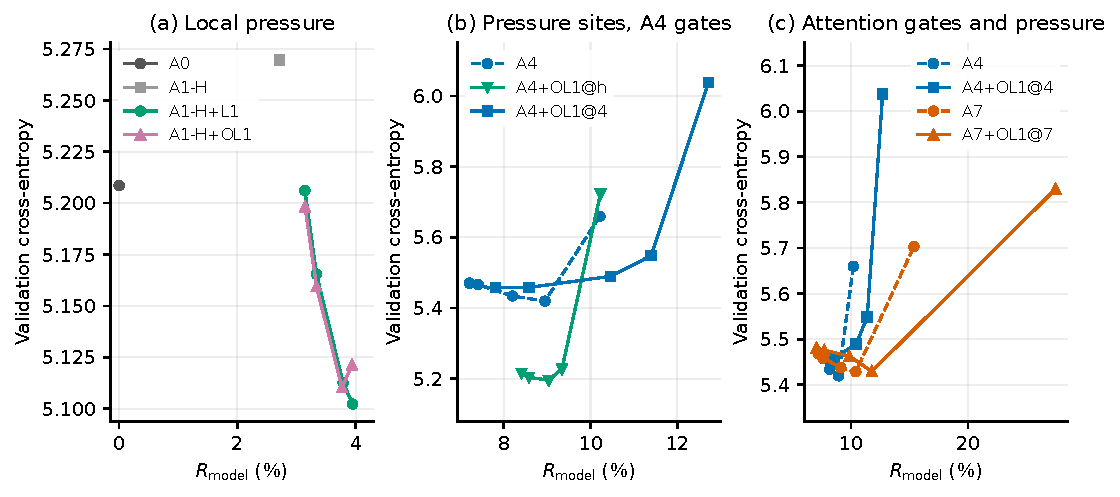
\includegraphics[width=\linewidth]{figures/01-matched-14m.pdf}
  \caption{Matched 14M intervention branches. Left: pressure on the feed-forward
  hidden state under a ReLU activation. Middle: four-site gating with pressure
  applied to zero, one, or four sites. Right: four- and seven-site gates, with
  and without pressure at their respective sites. Each line joins the tested
  pressure coefficients or gate thresholds. Lower loss and higher model-wide
  opportunity are preferred. Complete values and the negative pressure-site
  comparisons appear in Appendix~\ref{app:full-results}.}
  \label{fig:matched}
\end{figure}
% Evidence: analysis 013, observations/O001-matched-interventions.md; 01_build.py.

We evaluate opportunity as the fraction of scalar multiplications with an
exact-zero operand across the transformer blocks and dense output head.
This operation-weighted measure supports the intervention comparisons:
different gate sets affect different products, and the output head changes
the model-wide fraction across architectures. It complements validation loss
and measured latency.

Our contribution is an empirical account of how gate location and optimization
jointly shape the quality--sparsity frontier. It combines matched 14M
comparisons, a selected 70M extension of the pressured recipes, and
operation-level explanations of their gains and limits. The trained conditions
extend the evaluated uniform-clipping frontier, although clipping remains
competitive and is stronger under tight quality allowances at 70M.
We also report a negative 70M execution result and retain a fixed-budget
410M study in the appendix. Together, these observations distinguish an
improvement in learned sparsity from the additional structure and
implementation work required to turn it into faster inference.
